\section{Error Analysis}
\label{xsec:error_analysis}

We conduct a detailed error analysis of the best-performing model, GPT-4o. We randomly sample 97 errors and examine their distribution in detail. Based on this analysis, we classify the errors into five types, with the specific categories and their distribution shown in \Cref{fig:error_distribution}. Except for the \emph{Extractor Error} caused by our automatic evaluation pipeline, we present detailed definitions and descriptions of another six categories below:

\paragraph{Perceptual Error:} This category remains prevalent in complex document understanding tasks, where models frequently fail to accurately recognize, parse, or enumerate visual elements like tables, figures, and formulas in document screenshots. See \Cref{fig:perception_error_example_before_appendix} and \Cref{fig:perceptual_error_case2} for examples.

\paragraph{Reasoning Error:} Ranking as the third most prevalent error type, these failures occur during critical cognitive operations—including numerical calculations, comparative analyses, and content summarization—despite correct evidence retrieval. See \Cref{fig:reasoning_error_case1} for examples.

\paragraph{Inconsistent Format:} While our ground truth annotations strictly preserve original document content, GPT-4o sometimes generates outputs with formatting discrepancies. These variations principally involve: (1) abbreviation/full-form inconsistencies, (2) inclusion/omission of numerical units, and (3) mismatches in decimal precision. See \Cref{fig:inconsistent_format_case1} for examples.

\paragraph{Incomplete Evidence:} The LongDocURL benchmark reveals significant model limitations in processing extensive multimodal documents, where essential query-relevant information is sometimes omitted from responses. See \Cref{fig:incomplete_evidence_case1} for examples.

\paragraph{Irrelevant Answer:} Fundamental misinterpretations of query intent lead to responses that fail to address the actual information needs. See \Cref{fig:irrelevant_answer_case1} for examples.

\paragraph{Hallucinated Evidence:} The most severe error type involves model-generated fabrications, where non-existent document content is created to substantiate incorrect responses. See \Cref{fig:hallucinated_evidence_case1} for examples.

\begin{figure*}[!htbp]
    \centering
    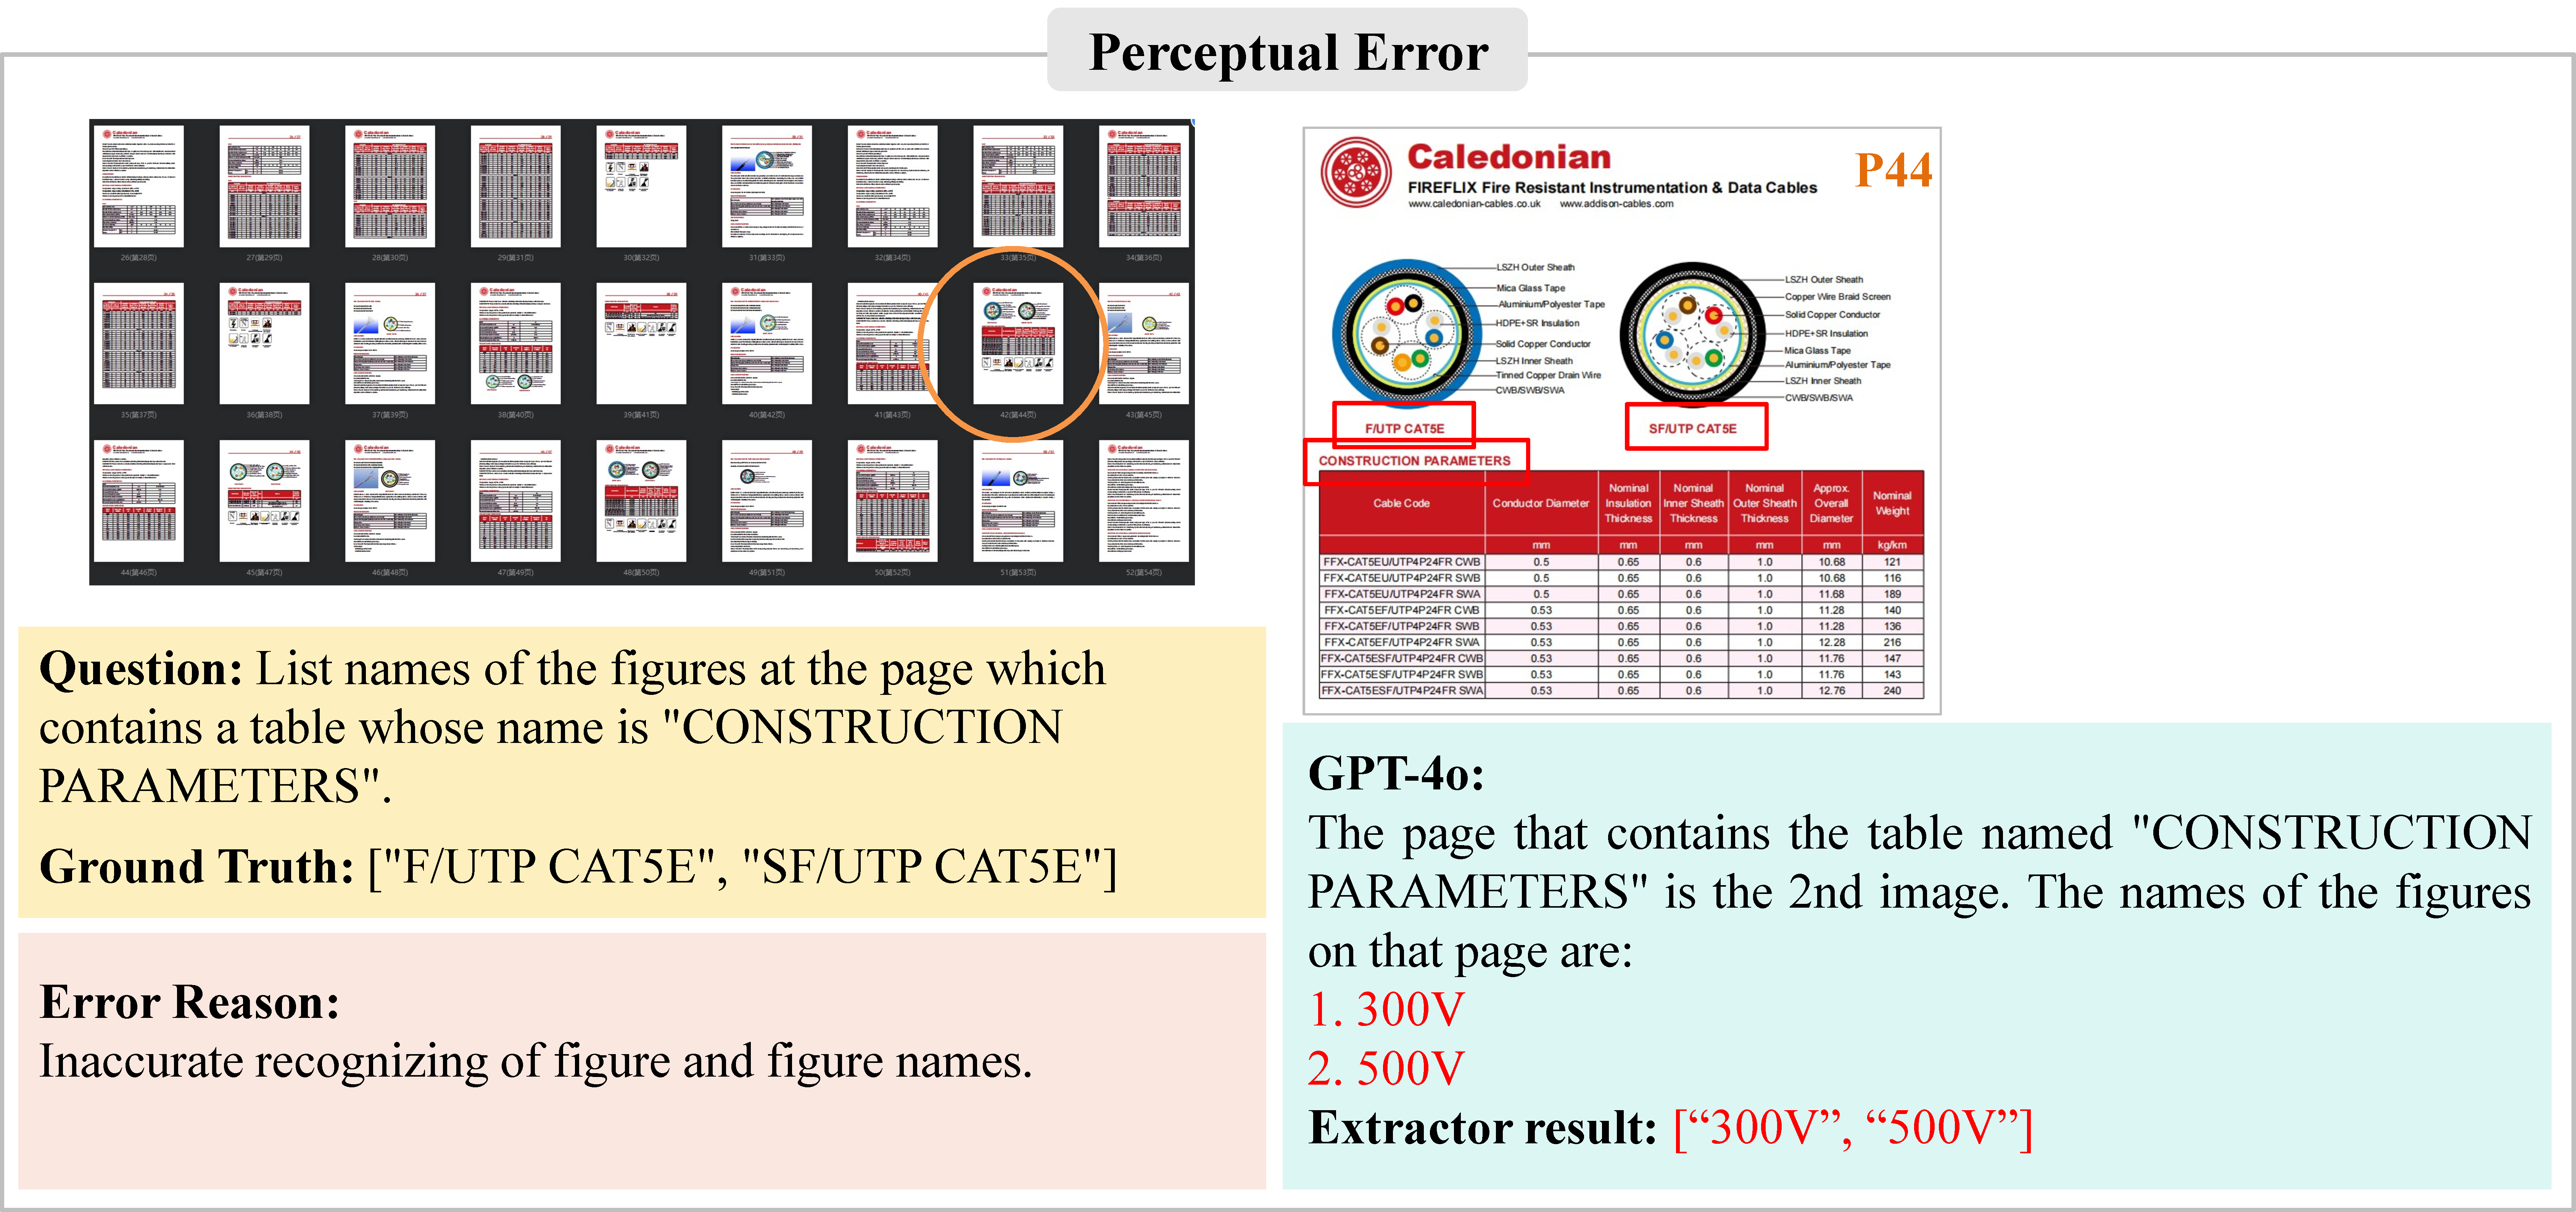
\includegraphics[width=1.0\textwidth]{img/perceptual_error_case2.pdf} % 调整宽度
    \caption{An example of \textit{Perceptual Error}.}
    \label{fig:perceptual_error_case2}
\end{figure*}

\begin{figure*}[!htbp]
    \centering
    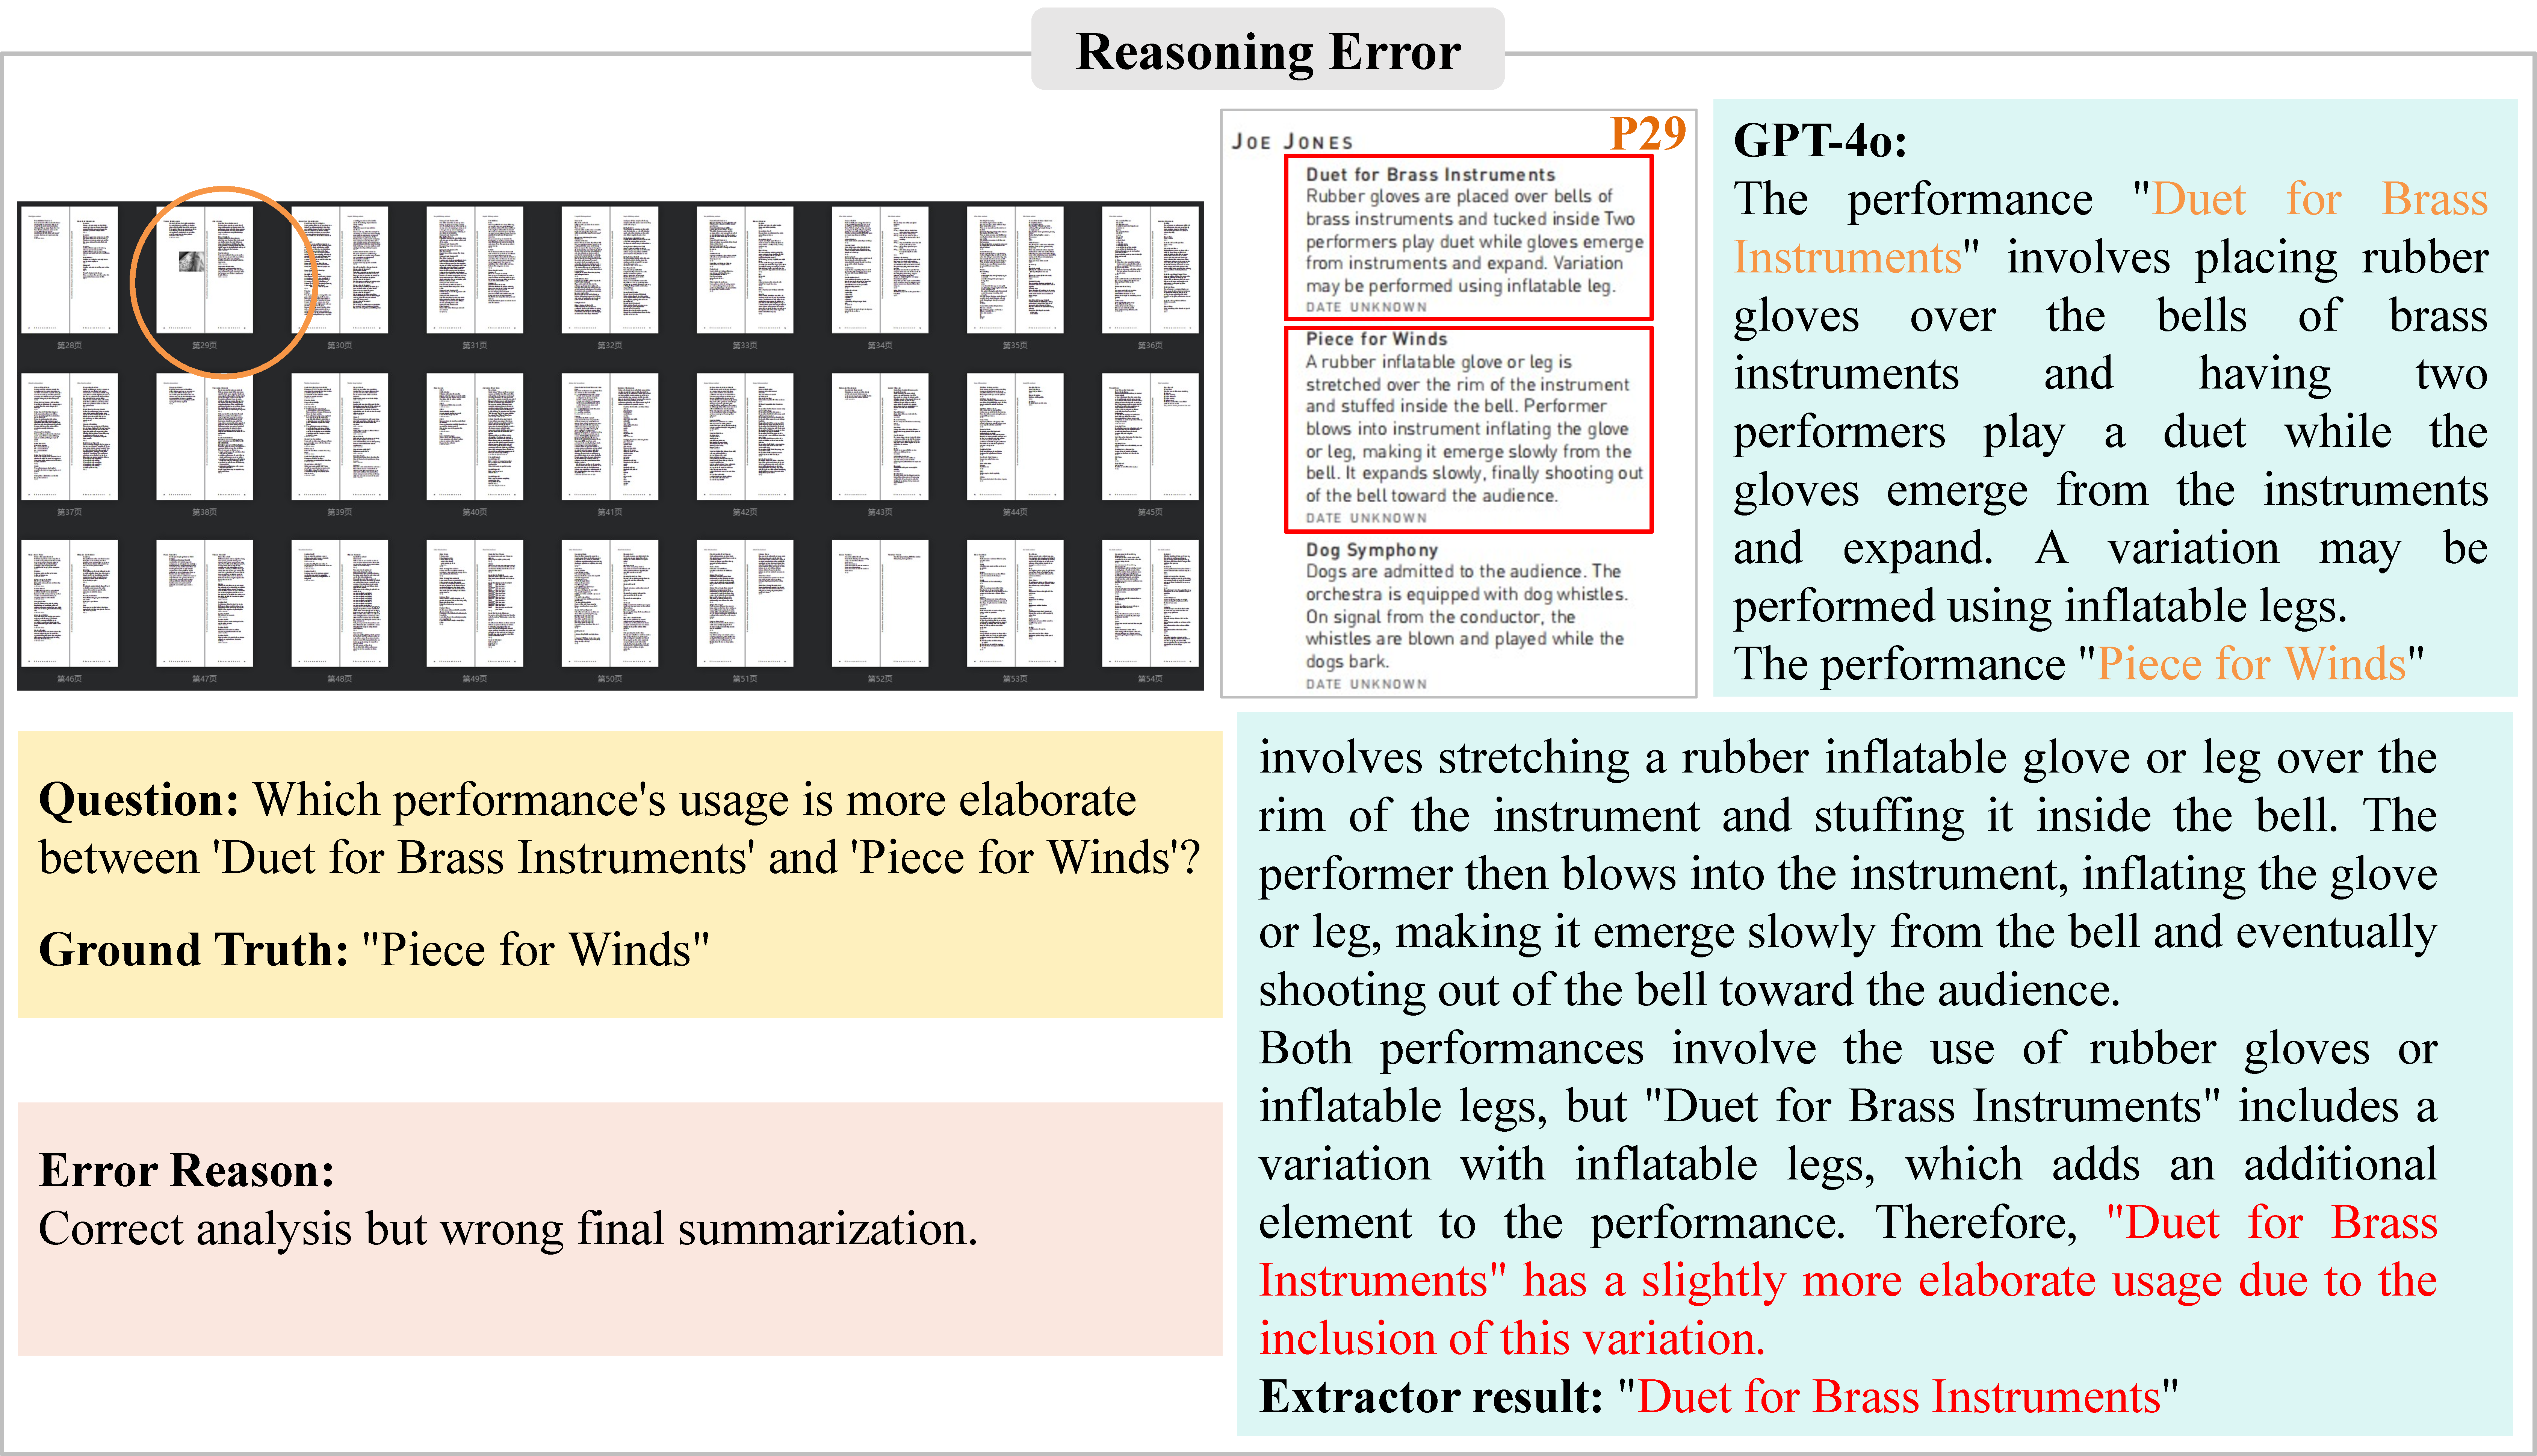
\includegraphics[width=1.0\textwidth]{img/reasoning_error_case1.pdf} % 调整宽度
    \caption{An example of \textit{Reasoning Error}.}
    \label{fig:reasoning_error_case1}
\end{figure*}

\begin{figure*}[!htbp]
    \centering
    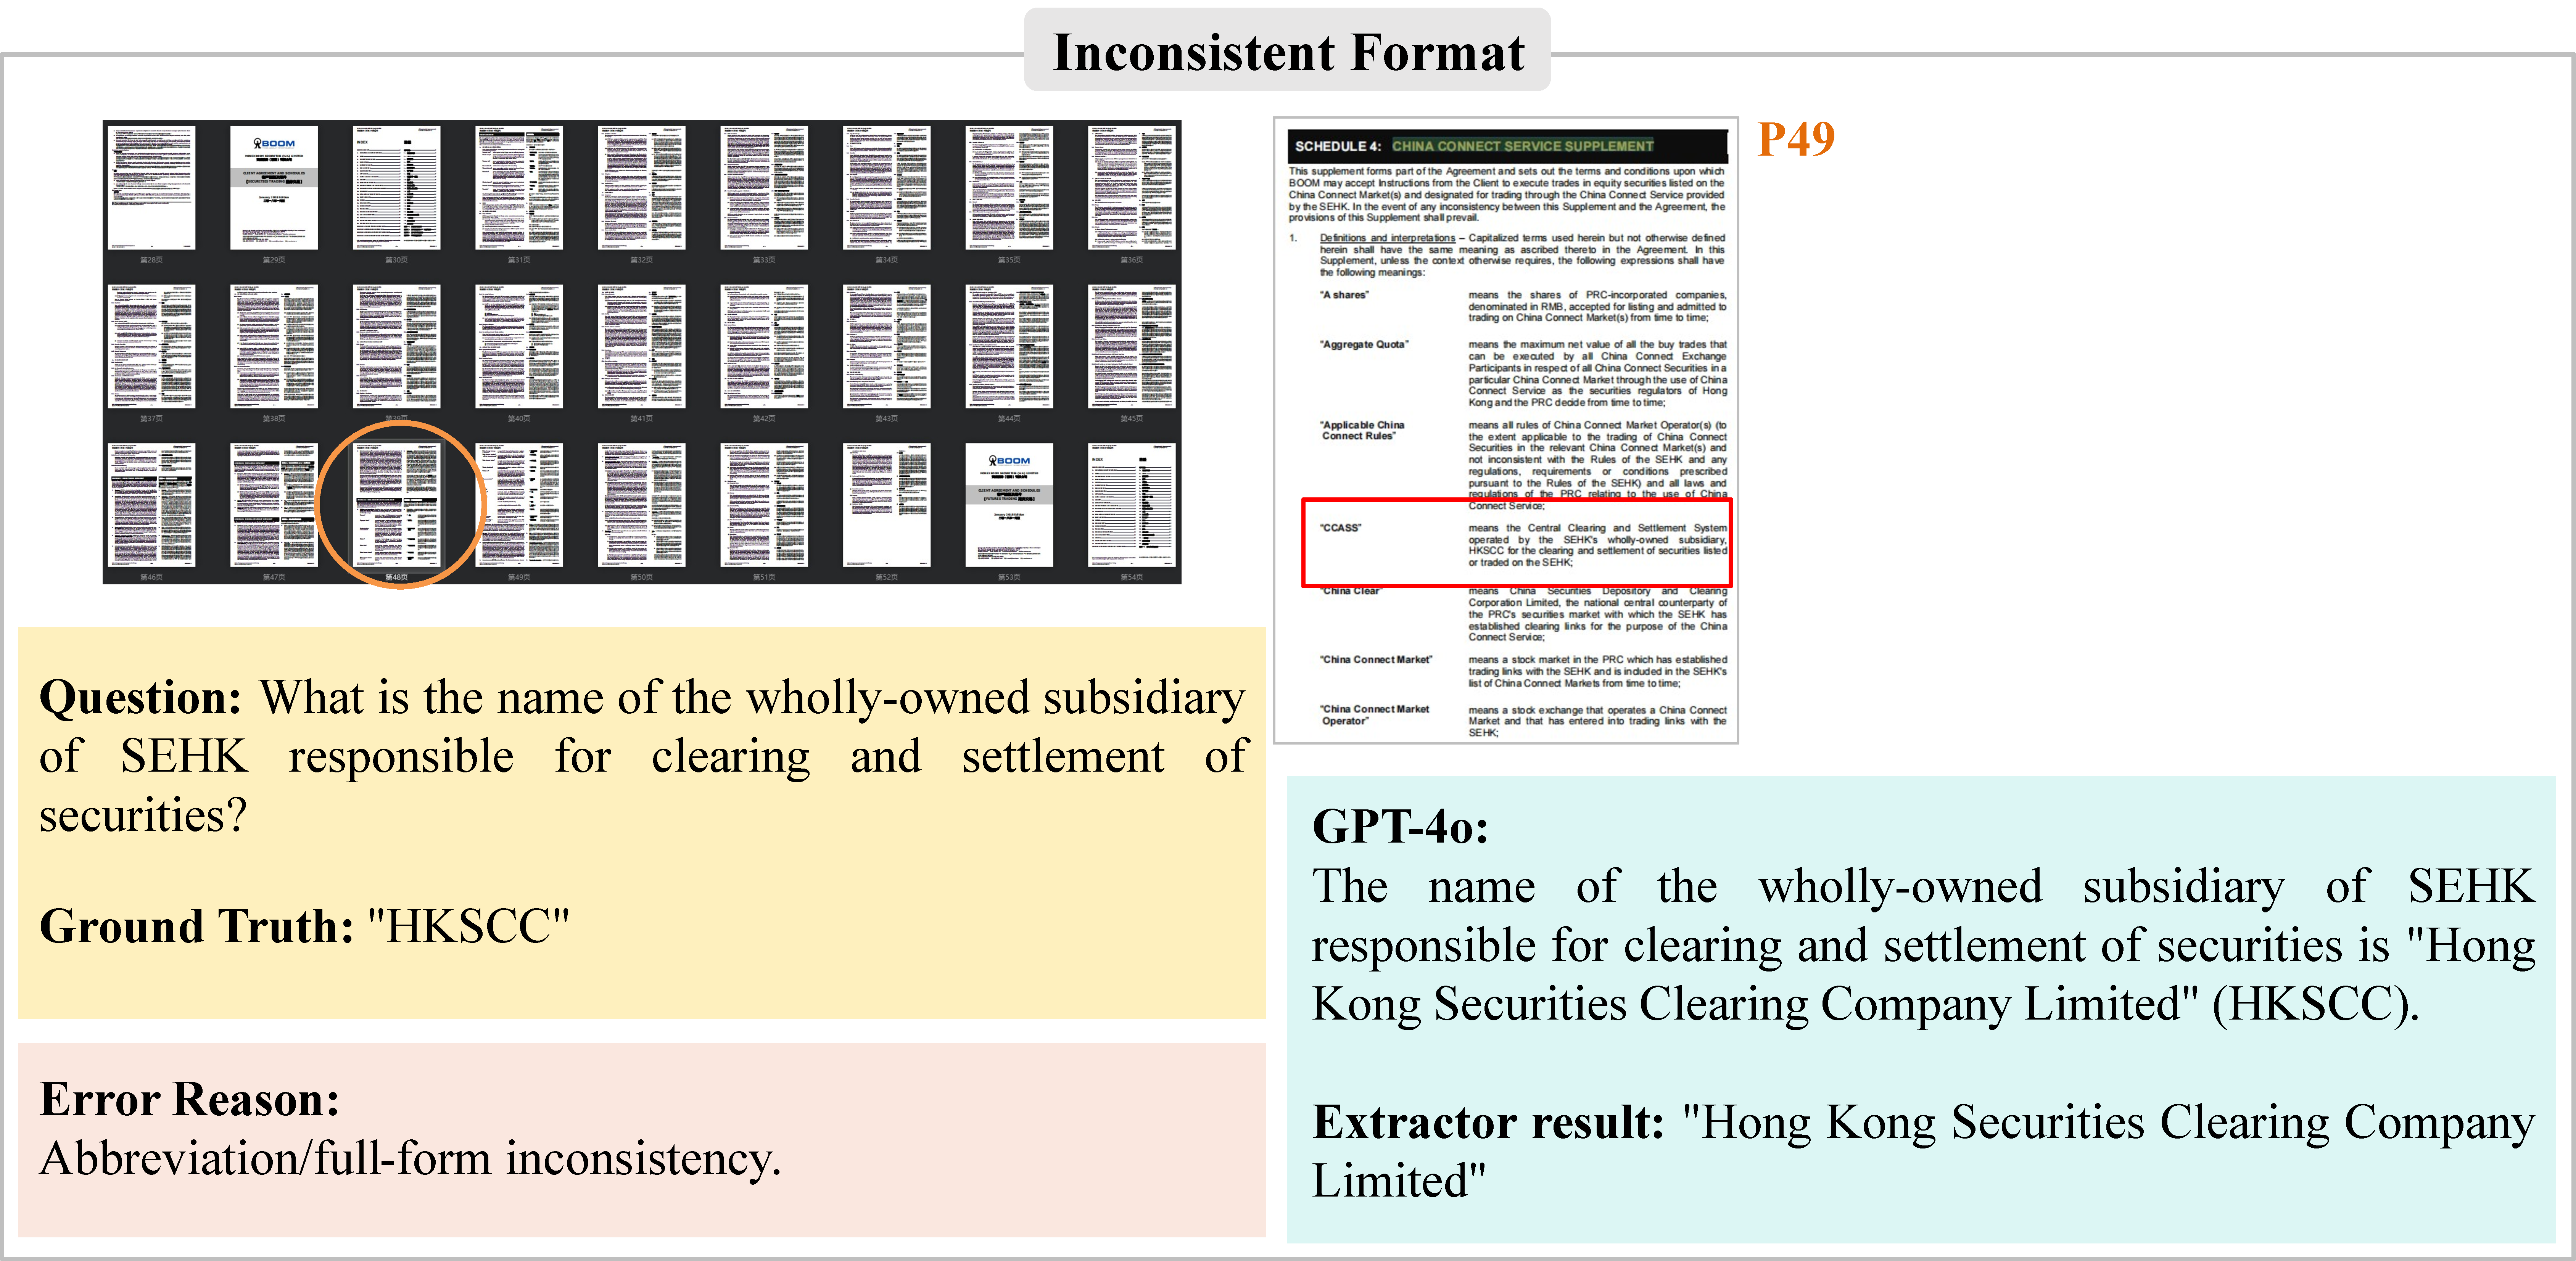
\includegraphics[width=1.0\textwidth]{img/inconsistent_format_case1.pdf} % 调整宽度
    \caption{An example of \textit{Inconsistent Format}.}
    \label{fig:inconsistent_format_case1}
\end{figure*}

\begin{figure*}[!htbp]
    \centering
    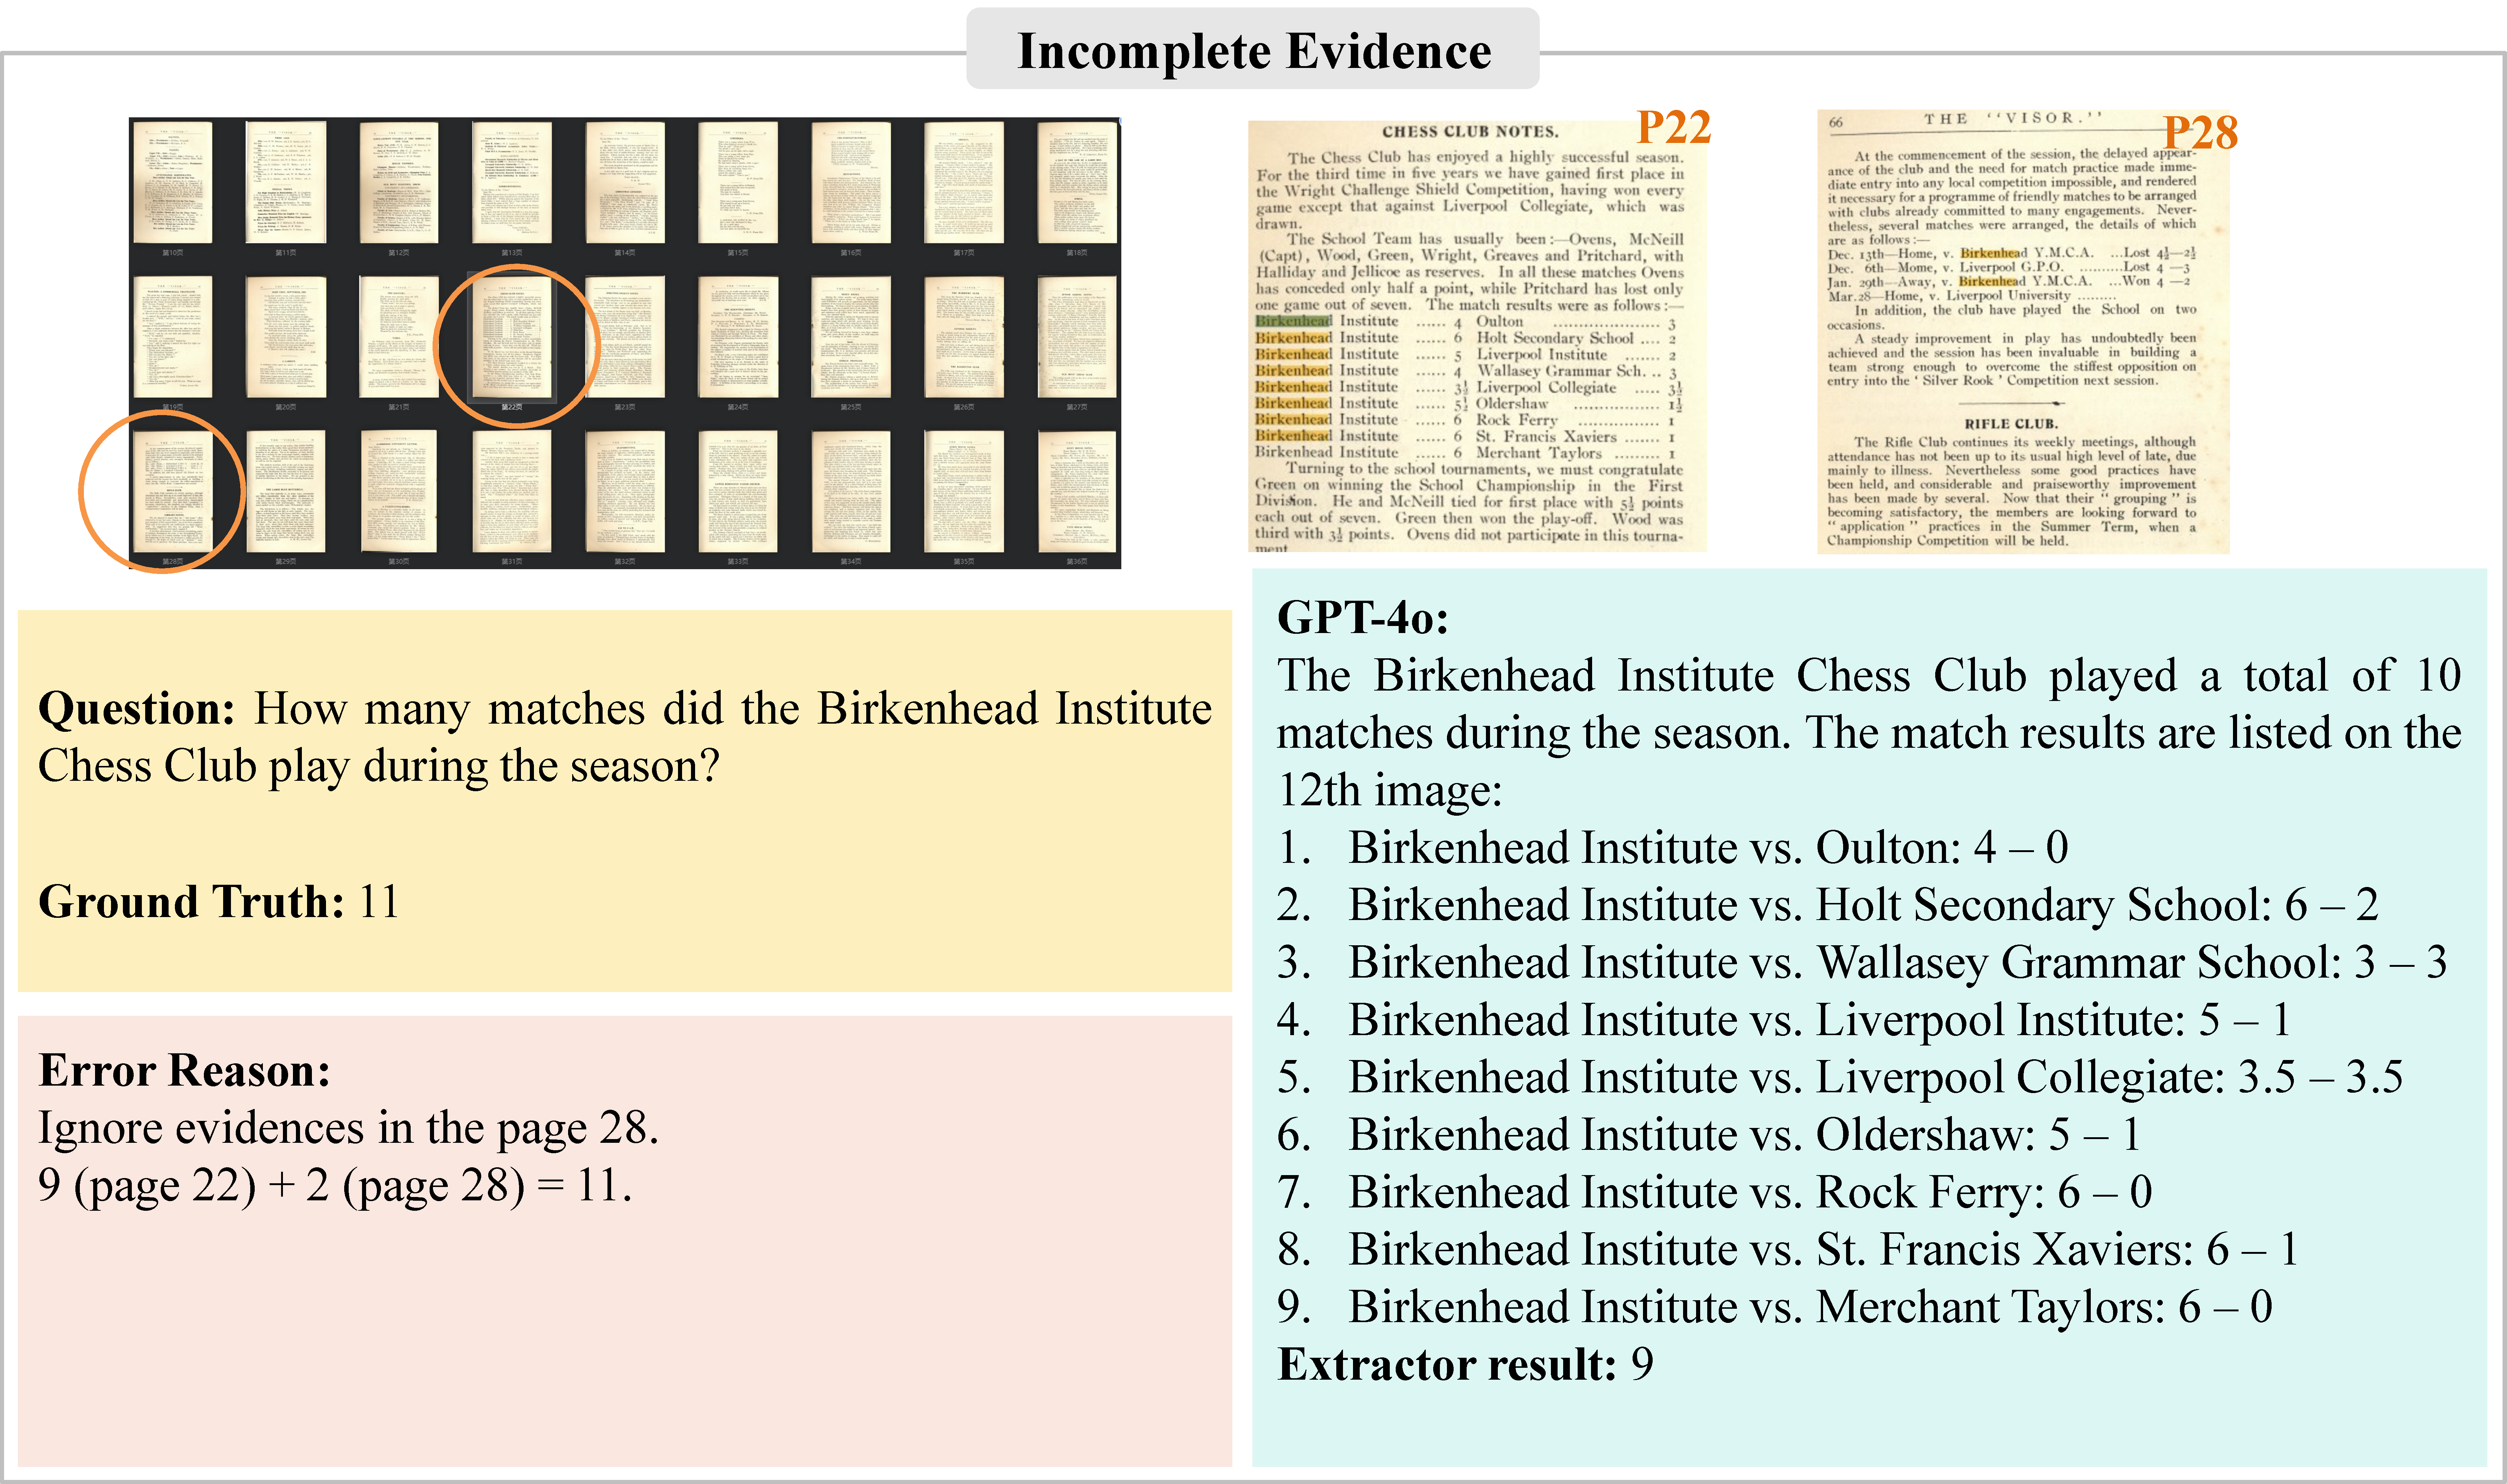
\includegraphics[width=1.0\textwidth]{img/incomplete_evidence_case1.pdf} % 调整宽度
    \caption{An example of \textit{Incomplete Evidence}.}
    \label{fig:incomplete_evidence_case1}
\end{figure*}

\begin{figure*}[!htbp]
    \centering
    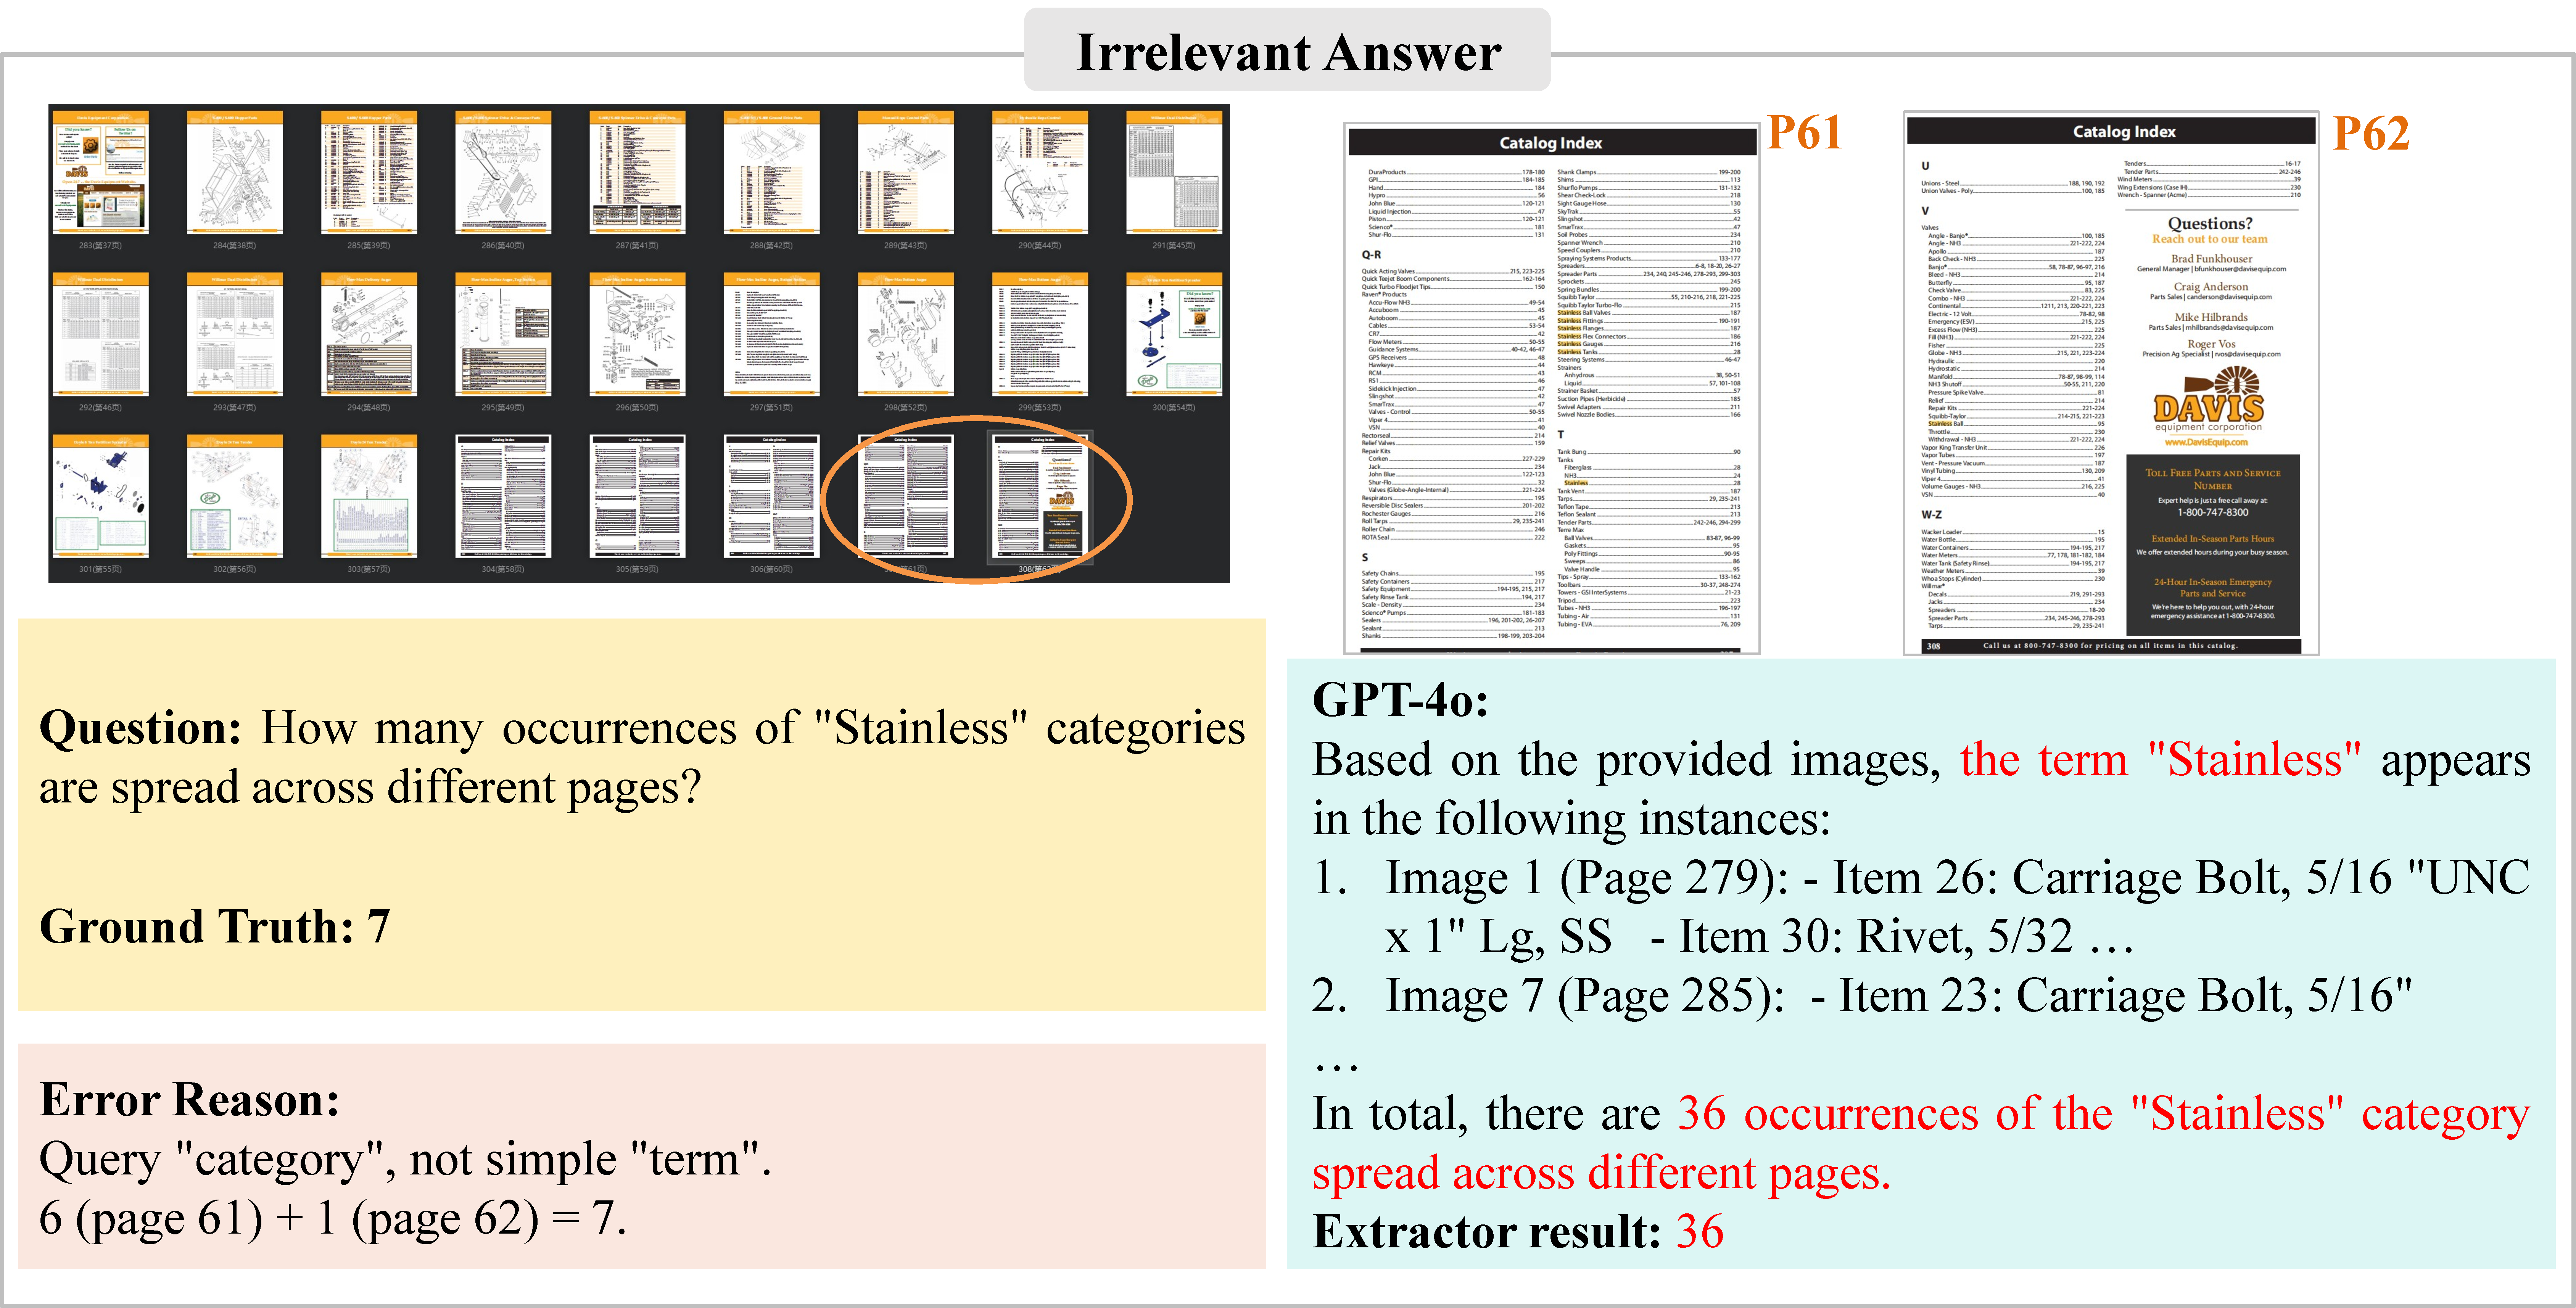
\includegraphics[width=1.0\textwidth]{img/irrelevant_answer_case1.pdf} % 调整宽度
    \caption{An example of \textit{Irrelevant Answer}.}
    \label{fig:irrelevant_answer_case1}
\end{figure*}

\begin{figure*}[!htbp]
    \centering
    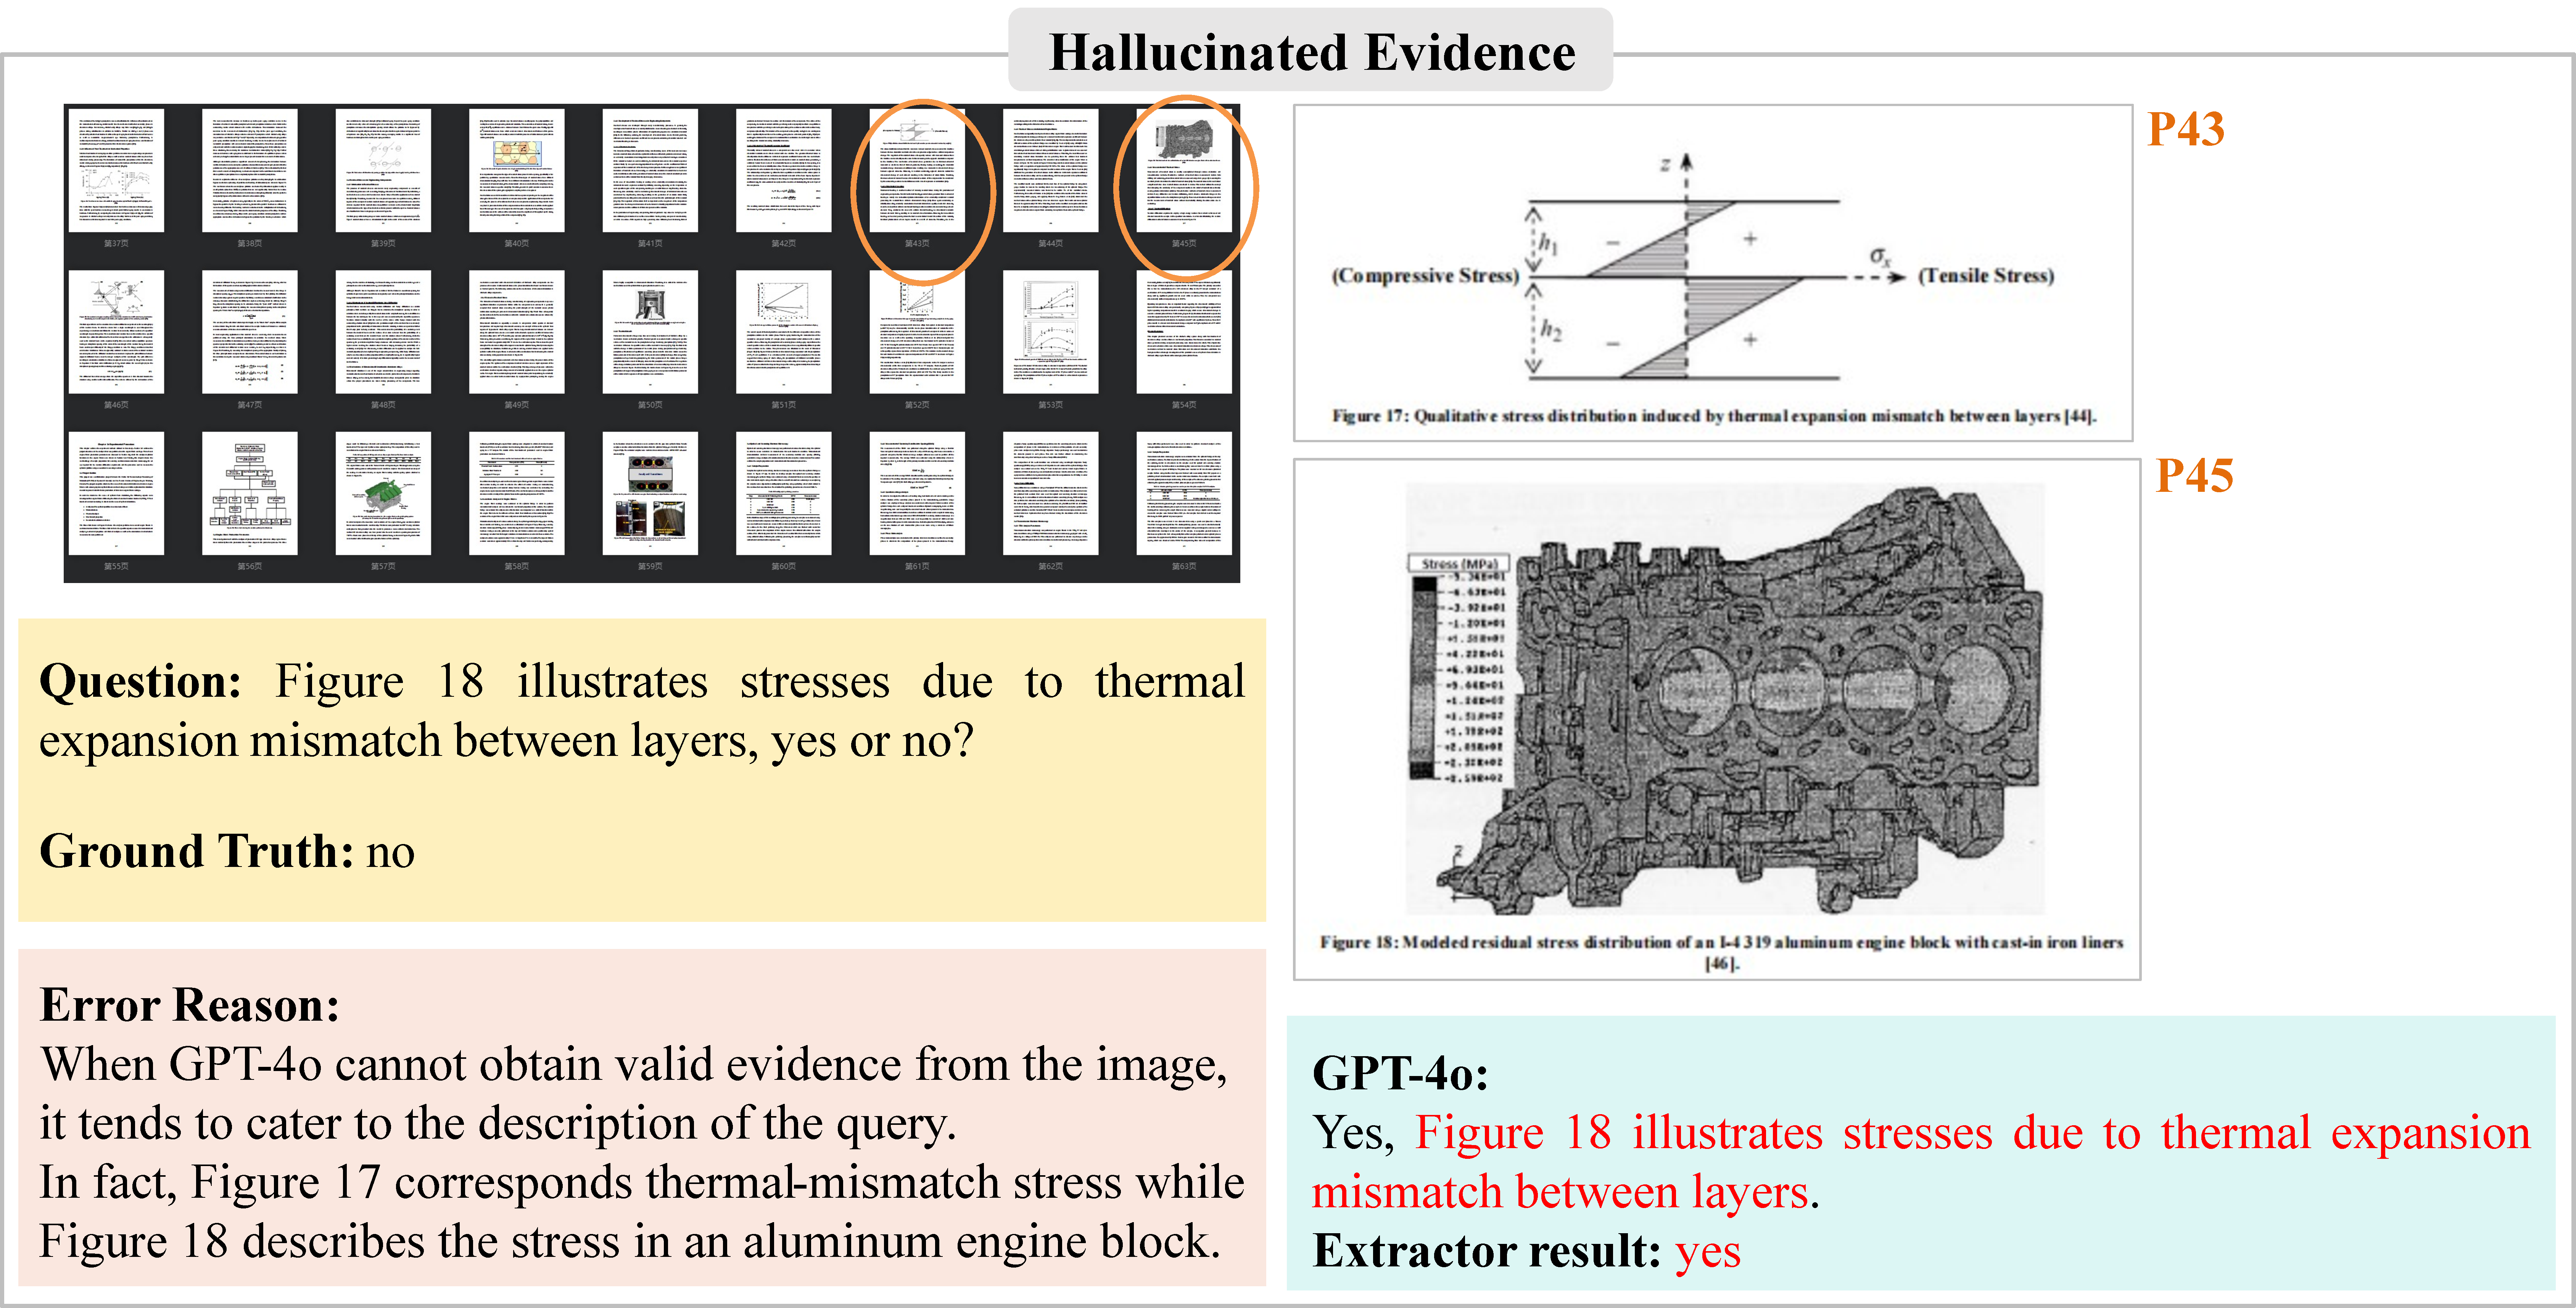
\includegraphics[width=1.0\textwidth]{img/hallucinated_evidence_case1.pdf} % 调整宽度
    \caption{An example of \textit{Hallucinated Evidence}.}
    \label{fig:hallucinated_evidence_case1}
\end{figure*}

